\graphicspath{{Chapter1/Figs/}}

\setcounter{chapter}{4}
\chapter*{Capítulo 1} 
\addcontentsline{toc}{chapter}{Capítulo 1}
\setcounter{figure}{0}
\setcounter{section}{0}


{\LARGE Aplicaciones bioinformáticas para el estudio de interacciones miARN-gen blanco}

\section{Introducción}
%~ Los miARNs son ARN pequeños de alrededor de 21 nucleótidos, son importantes reguladores de la expresión de genes en eucariotas y controlan procesos claves como el desarrollo y la respuesta a estrés.
%~ Los miARNs controlan la expresión génica ajustando los niveles finales de las proteínas o eliminando los transcriptos de ARN en la célula.
%~ La identidad de los genes blancos está especificada por la molécula de miARN, la cual reconoce una secuencia por complementariedad de bases. 

En plantas, los miARNs generalmente regulan más de un gen de una misma familia \citep{Jones-Rhoades2006}, así por ejemplo, miR319 regula a cinco factores de transcripción de la familia TCP, mientras que el miR172 hace lo mismo con seis factores de transcripción con dominio AP2.
A su vez, los miARNs conservados en plantas se encuentran generalmente codificados como pequeñas familias de genes que codifican ARN pequeños de secuencias similares o idénticas (Figura \ref{fig:variabilidad_maduro}).
En el caso de miR319, hay tres genes diferentes que codifican para miARNs similares, en dos casos son idénticos (ath-miR319a, ath-miR319b), mientras que un tercero difiere en la base 20 (ath-miR319c, Figura \ref{fig:variabilidad_maduro}). 

Una de las posibles ventajas de tener familias génicas con múltiples miembros es que proporciona flexibilidad en la manera en la que cada uno de ellos es regulado \citep{pmid21466971, pmid19699140}.
Estas diferencias pueden ser por variaciones en elementos regulatorios en los promotores o en las estructuras de los precursores de miARNs que llevan a eficiencias de procesamiento diferenciales \citep{pmid19699140}.

Por otro lado, las diferencias en las secuencias de los miARNs maduros podrían causar que miARNs de una misma familia regulen diferentes conjuntos de genes.
Esto se ha demostrado previamente para la superfamilia que incluye a los miARNs miR319 y miR159.
Estos dos miARNs son muy similares en secuencia, al punto que varios autores los consideran miembros de una misma familia \citep{Jones-Rhoades2006}.
Sin embargo ha sido demostrado que regulan genes diferentes \citep{Schwab2005517, pmid12931144,Palatnik2007}.
Así, mientras el miR319 puede reprimir la expresión de factores de transcripción de la familia TCP y MYB, diferencias de secuencia en 4 nucleótidos previenen la actividad del miR159 sobre los TCP \citep{Palatnik2007}.

La identificación de genes blanco regulados por miARNs en plantas es muy importante para poder conocer el rol de los miARNs.
En general esta identificación, se obtiene de diferentes estrategias computacionales donde tienen en cuenta la complementariedad con sus mensajeros blanco.
Uno de los mayores desafíos es predecir los genes regulados por estos ARN pequeños con una baja frecuencia de predicciones falsas.

A partir de interacciones miARN-ARNm blanco validadas experimentalmente, se han determinado algunos parámetros empíricos para la identificación de genes blanco.
Por un lado, el hecho de que determinados genes con un número de "mismatches" fuesen blancos de regulación por miARNs mientras que otros con igual número no, sugería que debían existir otros factores que afectaran la interacción de los miARN con los ARNm blanco.
A partir de aquí es que algunas estrategias tienen en cuenta la posición relativa de los mismatches \citep{Schwab2005517}.
Es por esto que se han utilizado otros enfoques para abordar este problema, por ejemplo el requerimiento de que el sitio complementario al miARN en los ARNm estuviera conservados entre genes homólogos de Arabidopsis y arroz.

Más recientemente se desarrolló una tecnología, en este caso experimental, conocida como "degradoma", que permite obtener el perfil global de los productos de degradación de los ARN mensajeros \citep{German2008,pmid18472421}.
Este enfoque permitió detectar in vivo y a nivel genómico la actividad de los miARNs al identificarse los productos de corte de los ARNm mediado por estos ARNs pequeños.
Dicha información es muy útil para la identificación de nuevos posibles blancos.

En esta parte de la Tesis se profundizó esta cuestión y se desarrolló un método bioinformático para la predicción de genes regulados por miARNs conservados en plantas.

\begin{figure}[htbp!] 
    \centering    
    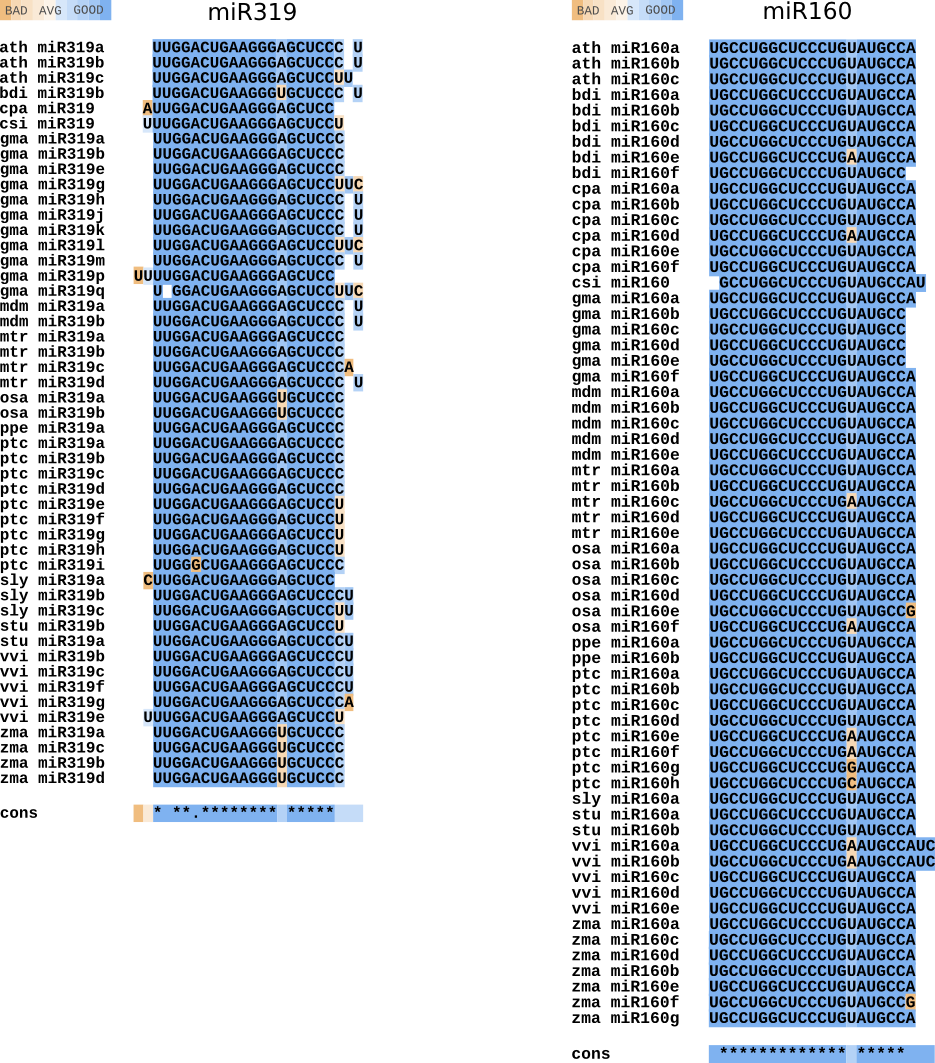
\includegraphics[width=0.7\textwidth]{variabilidad_maduro.png}
    \caption[Conservación y divergencia de miARNs en distintas especies]{
    \textbf{Conservación y divergencia de miARNs en distintas especies}
    Se muestra miembros de la familia del miR319 y del miR160 en distintas especies. 
    En colores se muestra la conservación de las bases  y el consenso (cons) se indica con asteriscos.
    Puede notarse que existe poca variabilidad de la secuencia del miARN maduro en distintas especies, pero aun así pueden observarse algunos cambios. 
		}
    \label{fig:variabilidad_maduro}
\end{figure}


\section{Resultados y Discusión}

%~ \subsection{Diseño de una estrategia para la identificación de genes blanco regulados por miARNs basado en la conservación evolutiva del par miARN-gen blanco.}
\subsection{Selección de secuencias de miARNs presentes en distintas especies}

Enfocamos nuestro análisis en 22 miARNs que están conservados en Angiospermas \citep{citeulike:8816489,10.1371/journal.pgen.1002419} (Tabla \ref{table:table_consensus}).
En general estos miARNs están codificados por pequeñas familias de hasta 32 miembros.
En los genomas completos de Arabidopsis, poplar y arroz es común encontrar variaciones en la secuencia de los miARNs pertenecientes a una misma familia, especialmente en el primer nucleótido y los nucleótidos 20 y 21 \citep{10.1371/journal.pgen.1002419}.

Sin embargo, observamos que la región entre la posición 2 y 19 está relativamente conservada y pudimos encontrar una secuencia consenso presente en la mayoría de los miembros de cada familia de miARNs en esas tres especies (Tabla \ref{table:table_consensus}).
Curiosamente, las bases variables fuera de esta región conservada son propensas a tener "mismatches" con genes blanco conocidos, lo que indica que podría existir una correlación entre la interacción miARN-gen blanco y la conservación de la secuencia del miARN.

Nos enfocamos entonces en estas secuencias de 18 nt (entre las posiciones 2 y 19) y en Arabidopsis, poplar y arroz que cuentan con sus genomas totalmente secuenciados.
Vimos que si consideramos a estas especies podíamos encontrar una secuencia consenso de 18 nt correspondiente a cada una de las 22 familias de miARNs conservados y que a su vez exista como tal en todas las especies (Tabla \ref{table:table_consensus}).
Dada la conservación de estas secuencias consenso de 18 nt en al menos estas tres especies distanciadas evolutivamente, y a que las bases de los extremos tienden a no interaccionar con las secuencias blanco, decidimos hacer nuestras búsquedas de blancos conservados evolutivamente con estos consensos.


\begin{table}
\tiny
\centering
\caption{miARNs y sus genes blanco en plantas}
\label{table:table_consensus}
\begin{tabular}{lllll}
\hline
\textbf{miARN} & \textbf{Consenso (18 nt)} & \textbf{Targets conocidos$^{(a,b)}$} &  &  \\ \hline
miR156 & GACAGAAGAGAGTGAGCA & factores de transcripción SPL&  &  \\
miR159 & TTGGATTGAAGGGAGCTC & factores de transcripción MYB, \textbf{NOZZLE (NZL)}&  &  \\
miR160 & GCCTGGCTCCCTGTATGC & factores de transcripción ARF&  &  \\
miR162 & CGATAAACCTCTGCATCC & DCL1&  &  \\
miR164 & GGAGAAGCAGGGCACGTG & factores de transcripción NAC&  &  \\
miR166 & CGGACCAGGCTTCATTCC & factores de transcripción HDZip&  &  \\
miR167 & GAAGCTGCCAGCATGATC & factores de transcripción ARF, \textbf{IAA-ALANINE RESISTANT 3 (IAR3)}&  &  \\
miR168 & CGCTTGGTGCAGGTCGGG & AGO1&  &  \\
mir169 & AGCCAAGGATGACTTGCC & factores de transcripción CCAAT-HAP2&  &  \\
mir171 & TTGAGCCGTGCCAATATC & factores de transcripción GRAS&  &  \\
miR172 & GAATCTTGATGATGCTGC & factores de transcripción AP2&  &  \\
miR319 & TGGACTGAAGGGAGCTCC & factores de transcripción TCP&  &  \\
miR390 & AGCTCAGGAGGGATAGCG & TAS RNA&  &  \\
miR393 & CCAAAGGGATCGCATTGA & TIR1 proteins, F-BOX proteins&  &  \\
miR394 & TGGCATTCTGTCCACCTC & proteínas F-BOX &  &  \\
miR395 & TGAAGTGTTTGGGGGAAC & ATP-sulfurilasas, transportadores de sulfato&  &  \\
miR396 & TCCACAGCTTTCTTGAAC & factores de transcripción GRF, \textbf{MMG4.7, FLUORESCENT IN BLUE LIGHT (FLU)}&  &  \\
miR397 & CATTGAGTGCAGCGTTGA & Laccases&  &  \\
miR398 & GTGTTCTCAGGTCACCCC & Cu/Zn SODs, CytC oxidase protein subunit, Chaperona de cobre (CCS)&  &  \\
miR399 & GCCAAAGGAGATTTGCCC & Enzima E2 de conjugación de ubiquitina&  &  \\
miR408 & TGCACTGCCTCTTCCCTG & Blue copper proteins, Laccases, \textbf{P-TYPE ATPase (PAA2), PAC1 (Proteasome component)}&  &  \\
miR827 & TAGATGACCATCAGCAAA & SPX proteins&  &  \\ \hline
\multicolumn{3}{l}{a Los genes blanco fueron agrupados según sus funciones.}\\
\multicolumn{3}{l}{b Nuevos genes blanco validados experimentalmente en este estudio están indicados en negrita.}\\

\end{tabular}
\end{table}


\subsection{Selección de las biblioteca de transcriptos de plantas}

Para estudiar la regulación por miARNs de genes en distintas especies vegetales, decidimos recurrir a la información disponible públicamente en el "Gene Index Project"\footnote{http://compbio.dfci.harvard.edu/tgi/}.
Este proyecto tiene los "contigs" de ESTs, de múltiples especies.
El proyecto es mantenido y administrado por la universidad de Harvard que contiene un catálogo completo de genes en una amplia gama de organismos incluyendo plantas.
En este proyecto las bibliotecas de EST (secuencias parciales de genes que se expresan) son ensambladas en "contigs" de tal manera de construir los ARNm que son expresados en las distintas especies.
Estas bibliotecas cuentan por lo tanto con transcriptos cuya expresión esta validada empíricamente.

De este catalogo de elegimos 41 especies de angiospermas (plantas con semillas) para hacer la búsqueda.
Además, utilizamos ARNm completos para las especies de \textit{A. thaliana} y \textit{Oryza Sativa}  que se encuentan caracterizados en detalle (para ver la lista completa de especies, ver tabla \ref{table:NAR_table_S2}).

\subsection{Primera búsqueda general de potenciales genes blanco}
Utilizando las secuencias consenso de 18nt y permitiendo 3 "mismatches" (Tabla \ref{table:table_consensus}), la búsqueda de genes blanco en las 43 especies seleccionadas (Tabla \ref{table:NAR_table_S2}) arrojó como resultado 38.597 genes (Figura \ref{fig:NAR_fig1}, bin 1).
En esta búsquedas las interacciones G-U y los "bulges" fueron considerados como "mismatches" en esta primera búsqueda.
%~ Todos los genes blanco de  \textit{A. thaliana} conocidos hasta ese momento fueron identificados usando esta estrategia con la excepción de CSD2, un gen blanco del miR398 que contiene 4 mismatches (tabla \ref{table:NAR_table_S2}).

Teniendo en cuenta que la mayoría de los genes blanco arrojados presentan una escasa descripción del tipo genómica funcional, realizamos un BLASTx  contra el proteoma de \textit{A. thaliana}.
El "locus ID" obtenido como "best hit" se utilizó como "tag" (etiqueta) para identificar al candidato en distintas especies (Figura \ref{fig:NAR_fig1}).
A pesar que esta estrategia no necesariamente identifica el gen ortólogo de Arabidopsis, sirve como propósito de clasificación de cada potencial gen blanco de miARN.
Aunque la mayoría de los potenciales genes blanco pudieron ser fácilmente asignados con una etiqueta, algunos pocos casos, que incluye a los genes que representan ARNs no codificantes fueron perdidos en este paso.

Este enfoque permite la selección de los mejores candidatos basándose en la presencia de los genes blanco en un número distinto de especies.
Utilizando 4 especies como el mínimo de especies requeridas (ya que tiene una buena especificidad), dio como resultado 3.781 genes que corresponden a 533 etiquetas diferentes (Figura \ref{fig:NAR_fig1}, bin 2).

La búsqueda también se puede hacer en combinación con filtros empíricos de interacción par miARN-gen blanco que tienen en cuenta la energía de interacción y la posición de los "mismatches" (ver Materiales y métodos).
De los 38.597 candidatos iniciales, 9.375 pasan estos filtros (Figura \ref{fig:NAR_fig1}, bin 4).
Combinando filtros de energía y filtro de conservación evolutiva, la búsqueda arrojó como resultado 563 candidatos correspondientes a 146 etiquetas (Figura \ref{fig:NAR_fig1}, bin 5).


\begin{figure}[htbp!] 
    \centering    
    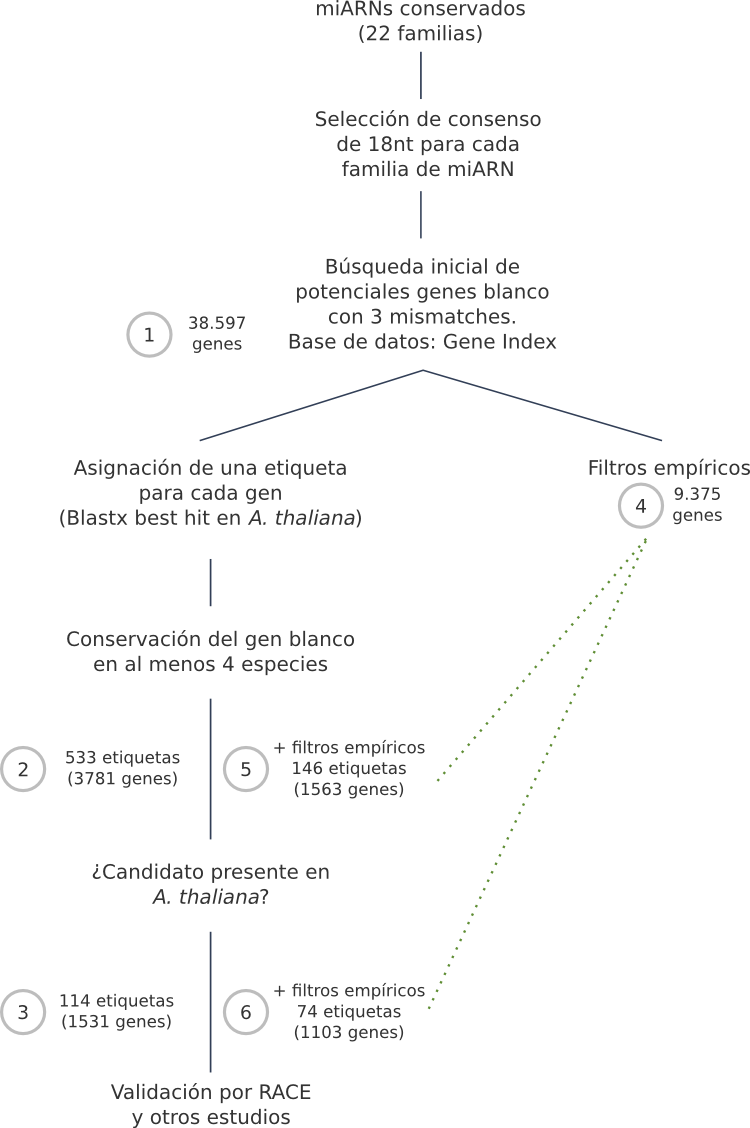
\includegraphics[width=0.7\textwidth]{NAR_fig1.png}
    \caption[Estrategia]{
    \textbf{Esquema de la estrategia para la identificación de nuevos genes blanco.}
    El número de genes blanco está identificado en cada paso. 
    Luego de aplicar el análisis de conservación, todos los genes que tienen el mismo hit en Arabidopsis, fueron considerados como un solo gen blanco. 
    El lado derecho muestra la búsqueda hecha con filtros empíricos: bin 5 y 6 incluyen genes blanco seleccionados con ambos filtros, empíricos y de conservación.
    Mientras que el bin 2 y 3 muestra los potenciales genes blanco seleccionados sólo con el filtro de conservación.}
    \label{fig:NAR_fig1}
\end{figure}




\subsection{Parámetros empíricos y de conservación evolutiva pueden actuar de manera sinérgica para identificar genes blanco regulados por miARNs.}
Potenciales genes blanco de miARNs fueron clasificados de acuerdo al mínimo número de especie en donde fueron detectados (Figura 2A-E).
Como control para cada miARN generamos 10 secuencias "scramble" (al azar), dividiendo las secuencias originales de a di-nucleótidos y luego generando nuevas secuencias al azar conservando la composición de los di-nucleótidos.
Estas secuencias al azar fueron utilizadas para realizar búsqueda de genes blanco del mismo modo que lo hicimos para las secuencias originales.
Luego, la relación señal/ruido fue calculada como el cociente entre el número de genes blanco para los miARNs y el número promedio obtenido de las secuencias al azar.
El radio fue de 1,2 para todos los miARNs juntos sin requerir conservación y esa relación incrementa con el número de especie en donde los genes blanco fueron detectados (Figura \ref{fig:NAR_fig2} A, recuadro). 
Los datos para todos los miARNs y sus potenciales genes blanco conservados en al menos 4 especies están incluidos en la tabla \ref{table:NAR_table_2}.

Luego estudiamos la selección de candidatos teniendo en cuenta los filtros empíricos.
Para esto aplicamos una versión modificada de los filtros descritos anteriormente, y requiriendo (i) una energía mínima de hibridación (MFE) de al menos 72\% del apareamiento perfecto de cada secuencia consenso y (ii)  que sólo un "mismatch" pudiera estar presente entre la posición 1 y la 11 de la secuencia consenso (2-12 del miARN).
De la búsqueda inicial 9.375 genes pasaron estos filtros conteniendo el 97\% de los genes validados anteriormente de Arabidopsis. (Figura \ref{fig:NAR_fig1}, bin 4). 

Al aplicar solamente este filtro empírico, dio como resultado una relación señal/ruido de 1,7 cuando agrupamos todos los miARNs juntos (Figura \ref{fig:NAR_fig2} A).
Observamos que aplicar simultáneamente los filtros empíricos y de conservación aumentó significativamente la relación señal/ruido para todos los miARNs juntos (Figura \ref{fig:NAR_fig2} A recuadro) y también de cada miARN individualmente (Figura \ref{fig:NAR_fig2} B-E, recuadros y tabla \ref{table:NAR_table_2}).
En varios casos, esta relación es de hasta 10 veces cuando se requiere de que el gen blanco este presente en más de 5 especies y que pase los filtros empíricos (Figure \ref{fig:NAR_fig2} A–D).
Este efecto sinérgico indica que el filtro de conservación evolutiva y los parámetros empíricos pueden estar seleccionando aspectos diferentes de la interacción miARN-gen blanco.

Observamos que el número de genes blanco candidato y la relación señal/ruido es variable entre los distintos miARNs.
El miR396 tiene la mayor cantidad de potenciales genes blanco, 92 de ellos presentes en al menos 4 especies y 26 de ellos pasan además los filtros empíricos (Tabla \ref{table:NAR_table_2} y Figura \ref{fig:NAR_fig2} B).
El miR408 y el miR398 también tienen un número alto de potenciales genes blanco y buenas relaciones de señal/ruido (Figura \ref{fig:NAR_fig2} C-D).

En contraste, ciertos miARNs como el miR162, miR168 y miR399 tienen un solo potencial gen blanco conservado en al menos 4 especies de acuerdo con nuestra búsqueda (Tabla \ref{table:NAR_table_2} y Figura \ref{fig:NAR_fig2} E).
Al menos en el caso del miR162 y del miR168 este resultado podría estar reflejando su rol específico en la regulación por retroalimentación de la biogénesis del miARN, ya que controlan los niveles de expresión DCL1 y AGO1 respectivamente \citep{Vazquez2004,Xie2003}.

Como control adicional para nuestra estrategia, realizamos la búsqueda de genes blanco del miR158 y miR173, que son miARNs presentes solamente en \textit{A. thaliana} y especies bien cercanas (17).
Como era esperado, estos miARNs no generaron más candidatos que sus versiones al azar (Tabla \ref{table:NAR_table_2} y Figura \ref{fig:NAR_fig2} F).

Luego chequeamos si los pares miARN-gen blanco altamente conservados tenían una interacción más fuerte que los que están presentes en pocas especies.
Para esto calculamos la energía mínima de hibridación para cada interacción detectada en nuestro trabajo. 
Observamos que los pares miARN-gen blanco presentes en muchas especies tienden a tener energía de interacción mayores que los que están presentes en menos especies (Figure \ref{fig:NAR_fig3} A).
De todos modos, la correlación no fue notoria y algunas interacciones miARN-gen blanco tuvieron una baja energía de hibridación (Figure \ref{fig:NAR_fig3} A).
Estos resultados muestran que una alta conservación podría no ser necesariamente equivalente a una fuerte interacción, la misma podría proporcionar una explicación para los efectos sinérgicos causados por los filtros de evolución y empíricos sobre la relación señal/ruido.

\begin{figure}[htbp!] 
    \centering    
    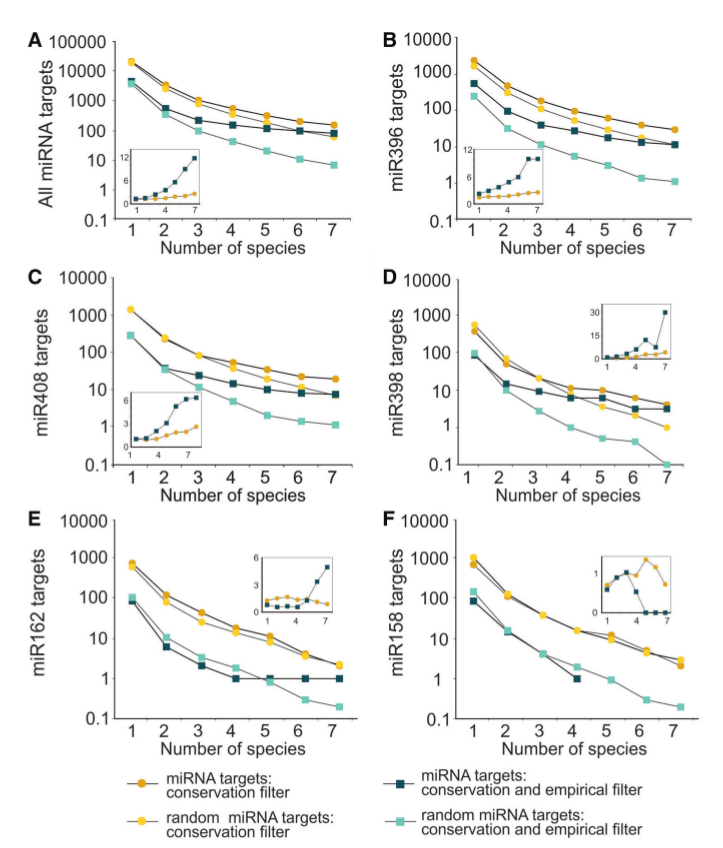
\includegraphics[width=0.9\textwidth]{NAR_fig2.png}
    \caption[Conservación de potenciales genes blanco en distintas especies]{\textbf{Conservación de potenciales genes blanco en distintas especies.}
    Todos los miARNs \textbf{(A)}, miR396 \textbf{(B)}, miR408 \textbf{(C)}, miR398 \textbf{(D)}, miR162 \textbf{(E)}, miR158 \textbf{(F)}.
    Puntos naranja representan los genes blanco de miARNs usando filtro evolutivo.
    Puntos amarillos representan los genes blanco de las secuencias al azar usando filtro evolutivo.
    El cuadrado azul muestra los genes blanco de miARNs luego de aplicar filtros empíricos y evolutivos, mientras que el cuadrado celeste representa los genes blanco de las secuencias al azar en las mismas condiciones.
    Los recuadros muestran la relación señal/ruido.}
    \label{fig:NAR_fig2}
\end{figure}

\begin{figure}[htbp!] 
    \centering    
    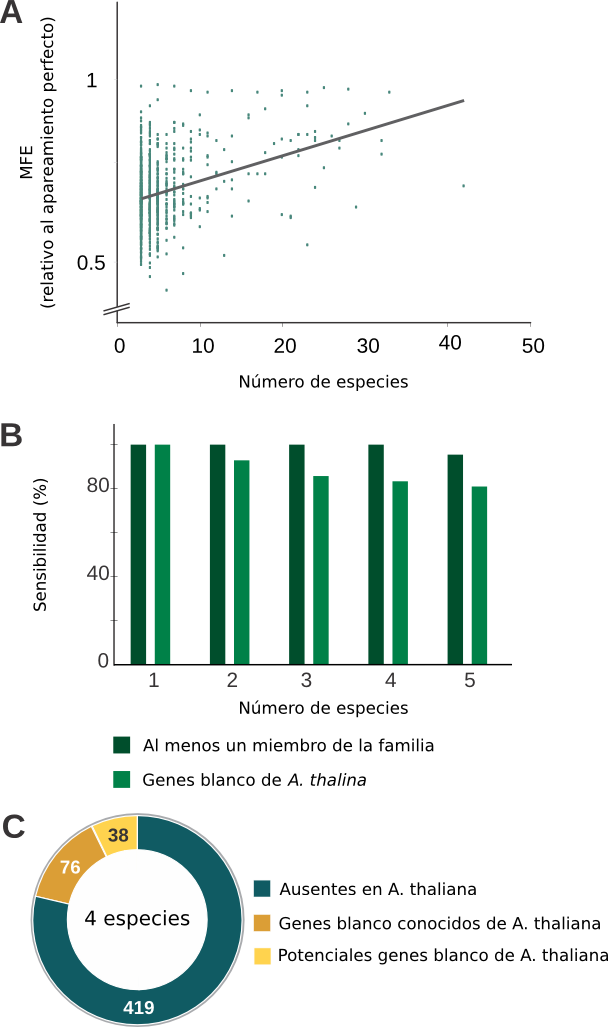
\includegraphics[width=0.6\textwidth]{NAR_fig3.png}
    \caption[Selección de genes blanco por conservación evolutiva de la secuencia]{
    \textbf{Selección de genes blanco por conservación evolutiva de la secuencia.}
    \textbf{(A)} Relación entre MFE y el número de especies en donde cada gen blanco fue detectado.
    \textbf{(B)} Sensibilidad de la estrategia, analizado de dos modos distinto. 
    Verde clarito: evaluando la presencia de genes validados en Arabidopsis y en verde oscuro teniendo en cuenta la presencia de por lo menos un gen blanco de cada familia regulada por miARNs.
    \textbf{(C)} Clasificación de los potenciales genes blanco presentes en al menos 4 especies.}
    \label{fig:NAR_fig3}
\end{figure}



\begin{landscape}
\begin{table}[]
\scriptsize
\centering
\caption{Detección de genes blanco de miARNs utilizando diferentes filtros}
\label{table:NAR_table_2}
\begin{tabular}{lllllllllllllllll}
\multicolumn{1}{c}{} & \multicolumn{4}{c}{\textbf{Sin filtros}}                        & \multicolumn{4}{c}{\textbf{Filtros empíricos}}                  & \multicolumn{4}{c}{\textbf{Conservación 4 especies}}            & \multicolumn{4}{c}{\textbf{Todos los filtros}}                  \\
\multicolumn{1}{c}{} & \multicolumn{1}{c}{\textbf{miARN}} & \multicolumn{1}{c}{\textbf{scramble}} & \multicolumn{1}{c}{\textbf{}} & \multicolumn{1}{c}{\textbf{ratio}} & \multicolumn{1}{c}{\textbf{miARN}} & \multicolumn{1}{c}{\textbf{scramble}} & \multicolumn{1}{c}{\textbf{}} & \multicolumn{1}{c}{\textbf{ratio}} & \multicolumn{1}{c}{\textbf{miARN}} & \multicolumn{1}{c}{\textbf{scramble}} & \multicolumn{1}{c}{\textbf{}} & \multicolumn{1}{c}{\textbf{ratio}} & \multicolumn{1}{c}{\textbf{miARN}} & \multicolumn{1}{c}{\textbf{scramble}} & \multicolumn{1}{c}{\textbf{}} & \multicolumn{1}{c}{\textbf{ratio}} \\
\textbf{miR156}      & 3915           & 3994.4            & $\pm$ 149.9     & 1.0            & 890            & 704.7             & $\pm$  45.2      & 1.3            & 34             & 39.7              & $\pm$  3.1       & 0.9            & 10             & 5.4               & $\pm$  1.1       & 1.9            \\
\textbf{miR159}      & 1663           & 1283.7            & $\pm$  47.8      & 1.3            & 472            & 254.9             & $\pm$  21.9      & 1.9            & 20             & 10.1              & $\pm$  1.1       & 2.0            & 6              & 1.5               & $\pm$  0.5       & 4.0            \\
\textbf{miR160}      & 793            & 695.6             & $\pm$  30.5      & 1.1            & 277            & 157.5             & $\pm$  28.8      & 1.8            & 5              & 4.4               & $\pm$  0.9       & 1.1            & 4              & 0.5               & $\pm$  0.3       & 8.0            \\
\textbf{miR162}      & 1191           & 930.2             & $\pm$  139.5     & 1.3            & 108            & 164.7             & $\pm$  24.1      & 0.7            & 18             & 13.5              & $\pm$  3.5       & 1.3            & 1              & 1.8               &  $\pm$ 0.5       & 0.6            \\
\textbf{miR164}      & 2486           & 1480.2            & $\pm$  60.4      & 1.7            & 678            & 333.2             & $\pm$  32.2      & 2.0            & 39             & 12.4              & $\pm$  1.9       & 3.1            & 12             & 1.5               & $\pm$  0.5       & 8.0            \\
\textbf{miR166}      & 879            & 815.5             & $\pm$  45.0      & 1.1            & 231            & 129               & $\pm$  14.5      & 1.8            & 16             & 10.6              & $\pm$  1.4       & 1.5            & 6              & 0.9               & $\pm$  0.4       & 6.7            \\
\textbf{miR167}      & 1777           & 1364.2            & $\pm$  146.6     & 1.3            & 478            & 214.8             & $\pm$  27.5      & 2.2            & 22             & 20.2              & $\pm$  3.6       & 1.1            & 4              & 1.8               & $\pm$  0.5       & 2.2            \\
\textbf{miR168}      & 962            & 797.5             & $\pm$  48.5      & 1.2            & 209            & 185               & $\pm$  14.2      & 1.1            & 6              & 4.4               & $\pm$  0.8       & 1.4            & 1              & 1.1               & $\pm$  0.5       & 0.9            \\
\textbf{miR169}      & 1540           & 1047.2            & $\pm$  69.7      & 1.5            & 464            & 181.4             & $\pm$  15.6      & 2.6            & 26             & 11.1              & $\pm$  2.1       & 2.3            & 10             & 1.2               & $\pm$  0.2       & 8.3            \\
\textbf{miR171}      & 884            & 723.4             & $\pm$  32.1      & 1.2            & 202            & 113.8             & $\pm$  13.4      & 1.8            & 7              & 6.6               & $\pm$  1.4       & 1.1            & 2              & 0.7               & $\pm$  0.3       & 2.9            \\
\textbf{miR172}      & 3007           & 1693.7            & $\pm$  124.7     & 1.8            & 540            & 288.1             & $\pm$  40.3      & 1.9            & 34             & 17.7              & $\pm$  1.7       & 1.9            & 5              & 2.2               & $\pm$  0.6       & 2.3            \\
\textbf{miR319}      & 1363           & 1274.2            & $\pm$  113.6     & 1.1            & 324            & 249.2             & $\pm$  22.3      & 1.3            & 18             & 15                & $\pm$  2.8       & 1.2            & 7              & 1.8               & $\pm$  0.5       & 3.9            \\
\textbf{miR390}      & 873            & 814.4             & $\pm$  64.3      & 1.1            & 335            & 173               & $\pm$  22.5      & 1.9            & 8              & 4.7               & $\pm$  1.2       & 1.7            & 3              & 0.7               & $\pm$  0.5       & 4.3            \\
\textbf{miR393}      & 986            & 844.6             & $\pm$  58.7      & 1.2            & 276            & 124.6             & $\pm$  11.1      & 2.2            & 14             & 7.1               & $\pm$  1.2       & 2.0            & 5              & 0.5               & $\pm$  0.2       & 10.0           \\
\textbf{miR394}      & 1569           & 1531.4            & $\pm$  57.5      & 1.0            & 188            & 237.1             & $\pm$  25.0      & 0.8            & 26             & 21.4              & $\pm$  2.2       & 1.2            & 3              & 2.9               & $\pm$  0.5       & 1.0            \\
\textbf{miR395}      & 1472           & 1226.7            & $\pm$  66.7      & 1.2            & 426            & 217.6             & $\pm$  16.5      & 2.0            & 11             & 8.8               & $\pm$  1.3       & 1.3            & 6              & 1.3               & $\pm$  0.3       & 4.6            \\
\textbf{miR396}      & 4641           & 2979.3            & $\pm$  246.6     & 1.6            & 1246           & 390.5             & $\pm$  38.8      & 3.2            & 92             & 51.4              & $\pm$  5.9       & 1.8            & 26             & 5.4               & $\pm$  1.0       & 4.8            \\
\textbf{miR397}      & 1426           & 1050.9            & $\pm$  27.9      & 1.4            & 368            & 236.5             & $\pm$  23.5      & 1.6            & 26             & 9.7               & $\pm$  0.8       & 2.7            & 10             & 1.6               & $\pm$  0.3       & 6.3            \\
\textbf{miR398}      & 935            & 834               & $\pm$  34.5      & 1.1            & 376            & 144               & $\pm$  18.1      & 2.6            & 11             & 7.5               & $\pm$  1.6       & 1.5            & 6              & 1                 & $\pm$  0.3       & 6.0            \\
\textbf{miR399}      & 1192           & 1137.6            & $\pm$  72.0      & 1.0            & 275            & 207.8             & $\pm$  24.9      & 1.3            & 5              & 13.6              & $\pm$  1.7       & 0.4            & 1              & 1.5               & $\pm$  0.7       & 0.7            \\
\textbf{miR408}      & 2782           & 2502.9            & $\pm$  103.6     & 1.1            & 695            & 468.7             & $\pm$  50.8      & 1.5            & 51             & 35.1              & $\pm$  3.0       & 1.5            & 14             & 4.6               & $\pm$  0.8       & 3.0            \\
\textbf{miR827}      & 2261           & 2000.1            & $\pm$  119.8     & 1.1            & 317            & 297.1             & $\pm$  45.0      & 1.1            & 44             & 23.4              & $\pm$  3.9       & 1.9            & 4              & 2.3               & $\pm$  0.8       & 1.7            \\
\textbf{Total}       & 38597          & 31021.7           & $\pm$  1859.8    & 1.2            & 9375           & 5473.2            & $\pm$  576.3     & 1.7            & 533            & 348.4             & $\pm$  47.0      & 1.5            & 146            & 42.2              & $\pm$  11.3      & 3.5            \\
\textbf{Control}     &                &                   &                  &                &                &                   & $\pm$            &                &                &                   &                  &                &                &                   &                  &                \\
\textbf{miR158}      & 1364           & 1462.8            & $\pm$  69.1      & 0.9            & 170            & 208.7             & $\pm$  15.8      & 0.8            & 15             & 16                & $\pm$  1.7       & 0.9            & 1              & 1.9               & $\pm$  0.4       & 0.5            \\
\textbf{miR173}      & 1386           & 1232.1            & $\pm$  101.7     & 1.1            & 243            & 215.6             & $\pm$  23.4      & 1.1            & 11             & 12                & $\pm$  2.4       & 0.9            & 1              & 1.5               & $\pm$  0.4       & 0.7           \\
\multicolumn{17}{l}{a Sin filtros, búsqueda inicial utilizando los miARN consenso de 18nt y 3 mismatches.}\\
\multicolumn{17}{l}{b Filtros empíricos, energía de al menos 72\% del apareamiento perfecto y 1 mismatch en la posición 2-12 del par miARN-gen blanco.}\\
\multicolumn{17}{l}{c Conservación del ID tag en al menos cuatro especies.}\\
\multicolumn{17}{l}{d Todos los filtros, combinación de los filtros empíricos y de conservación en al menos cuatro especies.}\\
\multicolumn{17}{l}{e miARN, genes blanco para cada miARN específico.}\\
\multicolumn{17}{l}{f scramble, promedio de los genes blanco de 10 versiones al azar de cada miARN ± error estándar.}\\
\end{tabular}
\end{table}
\end{landscape}

\subsection{Identificación de nuevos genes blanco en \textit{A. thaliana} por conservación de la secuencia del gen blanco.}


Para encontrar nuevos genes blanco nos enfocamos en los genes potenciales que fueron seleccionados de nuestra estrategia utilizando solamente conservación evolutiva, debido a que los parámetros empíricos ya fueron utilizados extensamente en trabajos anteriores. \citep{Allen2005207,JonesRhoades2004787,Schwab2005517}.
En primer lugar, analizamos la detección de genes blanco validados previamente en \textit{A. thaliana} [basado en \citep{Fahlgren2010}] usando nuestra estrategia y encontramos que el 84\% de ellos estaban presentes en al menos 4 especies (Figura \ref{fig:NAR_fig3} B).
Consideramos esto como un buen resultado ya que puede ser que no todos los genes blanco de Arabidopsis estén conservados evolutivamente.

Generalmente los miARNs en plantas regulan genes que codifican para proteínas de la misma familia, es por esto que evaluamos si por lo menos un miembro de cada familia era detectado en nuestro enfoque.
Encontramos genes blanco pertenecientes a casi todas las familias de genes codificantes para proteínas presentes en cuatro especies (Figura \ref{fig:NAR_fig3} B), con la excepción de TAS3, que es regulado por el miR390, al ser un ARN no codificante no es detectado por Blastx. 

Para encontrar nuevos genes blanco regulados por miARNs, nos enfocamos únicamente  en los potenciales genes blanco conservados en 4 especies, donde una de ellas es \textit{A. thaliana} (Figura 1, bin 1). 
Genes blanco de miARNs que no están presentes en \textit{A. thaliana} podrían incluir genes que perdieron su regulación durante la evolución o genes que hayan adquirido control por un miARN conservado más reciente en otras especies.
La conservación en cuatro especies fue elegida como un filtro evolutivo porque provee buena sensibilidad para genes blanco conocidos.

Identificamos 114 potenciales genes que satisfacen este criterio. Donde 76 de ellos son genes validados anteriormente o genes muy relacionados (Figura \ref{fig:NAR_fig3} C).
Curiosamente encontramos 38 genes que no tienen relación con genes blanco conocidos de miARNs y decidimos estudiar este grupo con mayor detalle.
Nos enfocamos primero en los genes que estaban presentes en un gran número de especies para tener mejor especificidad (Figura \ref{fig:NAR_fig2}) e intentamos validarlos utilizando 5' RACE PCR modificada \citep{Llave2002,Kasschau2003}.

Un potencial gen blanco del MiR408 era At5g21930 que codifica para P-TYPE ATPase OF ARABIDOPSIS 2 (PAA2) y estaba presente en 22 especies distintas incluido monocotiledóneas y dicotiledóneas.
MiR408 es inusual debido a que tiene un 5'-A, sin embargo >30\% de las secuencias maduro del miR408 corresponden a una variante corrida 1 nt que empieza con 5'-U \citep{Maunoury2011} (Figura \ref{fig:NAR_fig4} A).
La validación experimental reveló fragmentos de ARNm compatible con este último sitio de corte (Figura \ref{fig:NAR_fig4} A). 
PAA2 es necesaria para el transporte de iones de cobre a plastocianina \citep{Niyogi2005}, y su regulación por el miR408 está relacionada con el rol de este miARN en la homeostasis de cobre \citep{Yamasaki2007}.

Otro potencial candidato del miR408 era At3g22110 que codifica para PROTEASOME ALPHA SUBUNIT C1 (PAC1) y estaba presente en 20 especies. Por medio de 5' RACE PCR demostramos que este gen es gen blanco del miR408 (Figura \ref{fig:NAR_fig4} A). 
Curiosamente la interacción del par miARN-gen blanco tiene 3 "mismatches" en la región 5', y se hubiera perdido como potencial gen blanco si se aplicaban solamente los filtros empíricos.

Luego estudiamos los genes blanco del miR396, donde los genes SVP y SUI1 estaban presentes en 29 y 19 especies respectivamente.
Pero en ambos casos fallamos al obtener producto de la PCR utilizando 5' RACE PCR modificada.
La falta de regulación de este gen por el miR396 podría estar relacionado a la débil energía de hibridación del par miARN-gen blanco, aunque no podemos descartar que el miR396 esté controlando su traducción.

Otros dos potenciales genes blanco del miR396 eran At5g43060 y At3g14110 que codifican para la proteasa MMG4.7 y FLUORESCENT IN BLUE LIGTH (FLU), respectivamente.
Y en ambos casos pudimos detectar el corte (Figura \ref{fig:NAR_fig4} C y D).
%~ Ver
%~ Determination of MMG4.7 and FLU transcript levels in 35S:miR396 plants revealed a significant decrease of FLU and a minor effect on MMG4.7


En contraste con el miR408 y miR396, donde tienen varios potenciales genes blanco, obtuvimos un solo potencial gen blanco para el miR159, un factor de transcripción MYB que regula desarrollo del estambre y polen \citep{Millar2005}.
El otro potencial gen blanco era At4g27330, conocido como NOZZLE/SPOROCYTLESS.
Este factor de trascripción, que participa en desarrollo del estambre y óvulo \citep{Biology1999,Yang1999}, fue también validado por 5' RACE PCR (Figura \ref{fig:NAR_fig4} E).
%~ Ver
%~ In good agreement, 35S:miR159 caused a reduction of both MYB and NOZZLE transcript levels (Supplementary Figure S2). A miR159 target with a NOZZLE-like domain has been also recently validated in tomato (51), which together with our results point toward a general role of miR159 in the regulation of NOZZLE-like genes. 
Es interesante notar que al menos las funciones de NOZZLE y PAA2 pueden estar directamente relacionadas con el rol de genes blanco, ya descritos anteriormente, del miR159 y miR408 respectivamente.

PAA2, FLU y NOZZLE fueron detectados en mono y dicotiledóneas mientras que PAC1 y MMG4.7 fueron detectadas solamente en dicotiledóneas (Figura \ref{fig:NAR_fig4} A-E).
Las posiciones del sitio de unión del miARN-gen blanco están altamente conservadas y muchas de las posiciones variables corresponden a "mismatches" con el miARN o variaciones del tipo G-C/G-U.
Además este método no requiere que el sitio del gen blanco esté conservada, sino más bien que haya una interacción predicha con el miARN en distintas especies.
De esta manera el sitio de NOZZLE, donde la secuencia cambia en diferentes especies (Figura \ref{fig:NAR_fig4} E), pudo ser detectado por este enfoque.

\begin{figure}[htbp!] 
    \centering    
    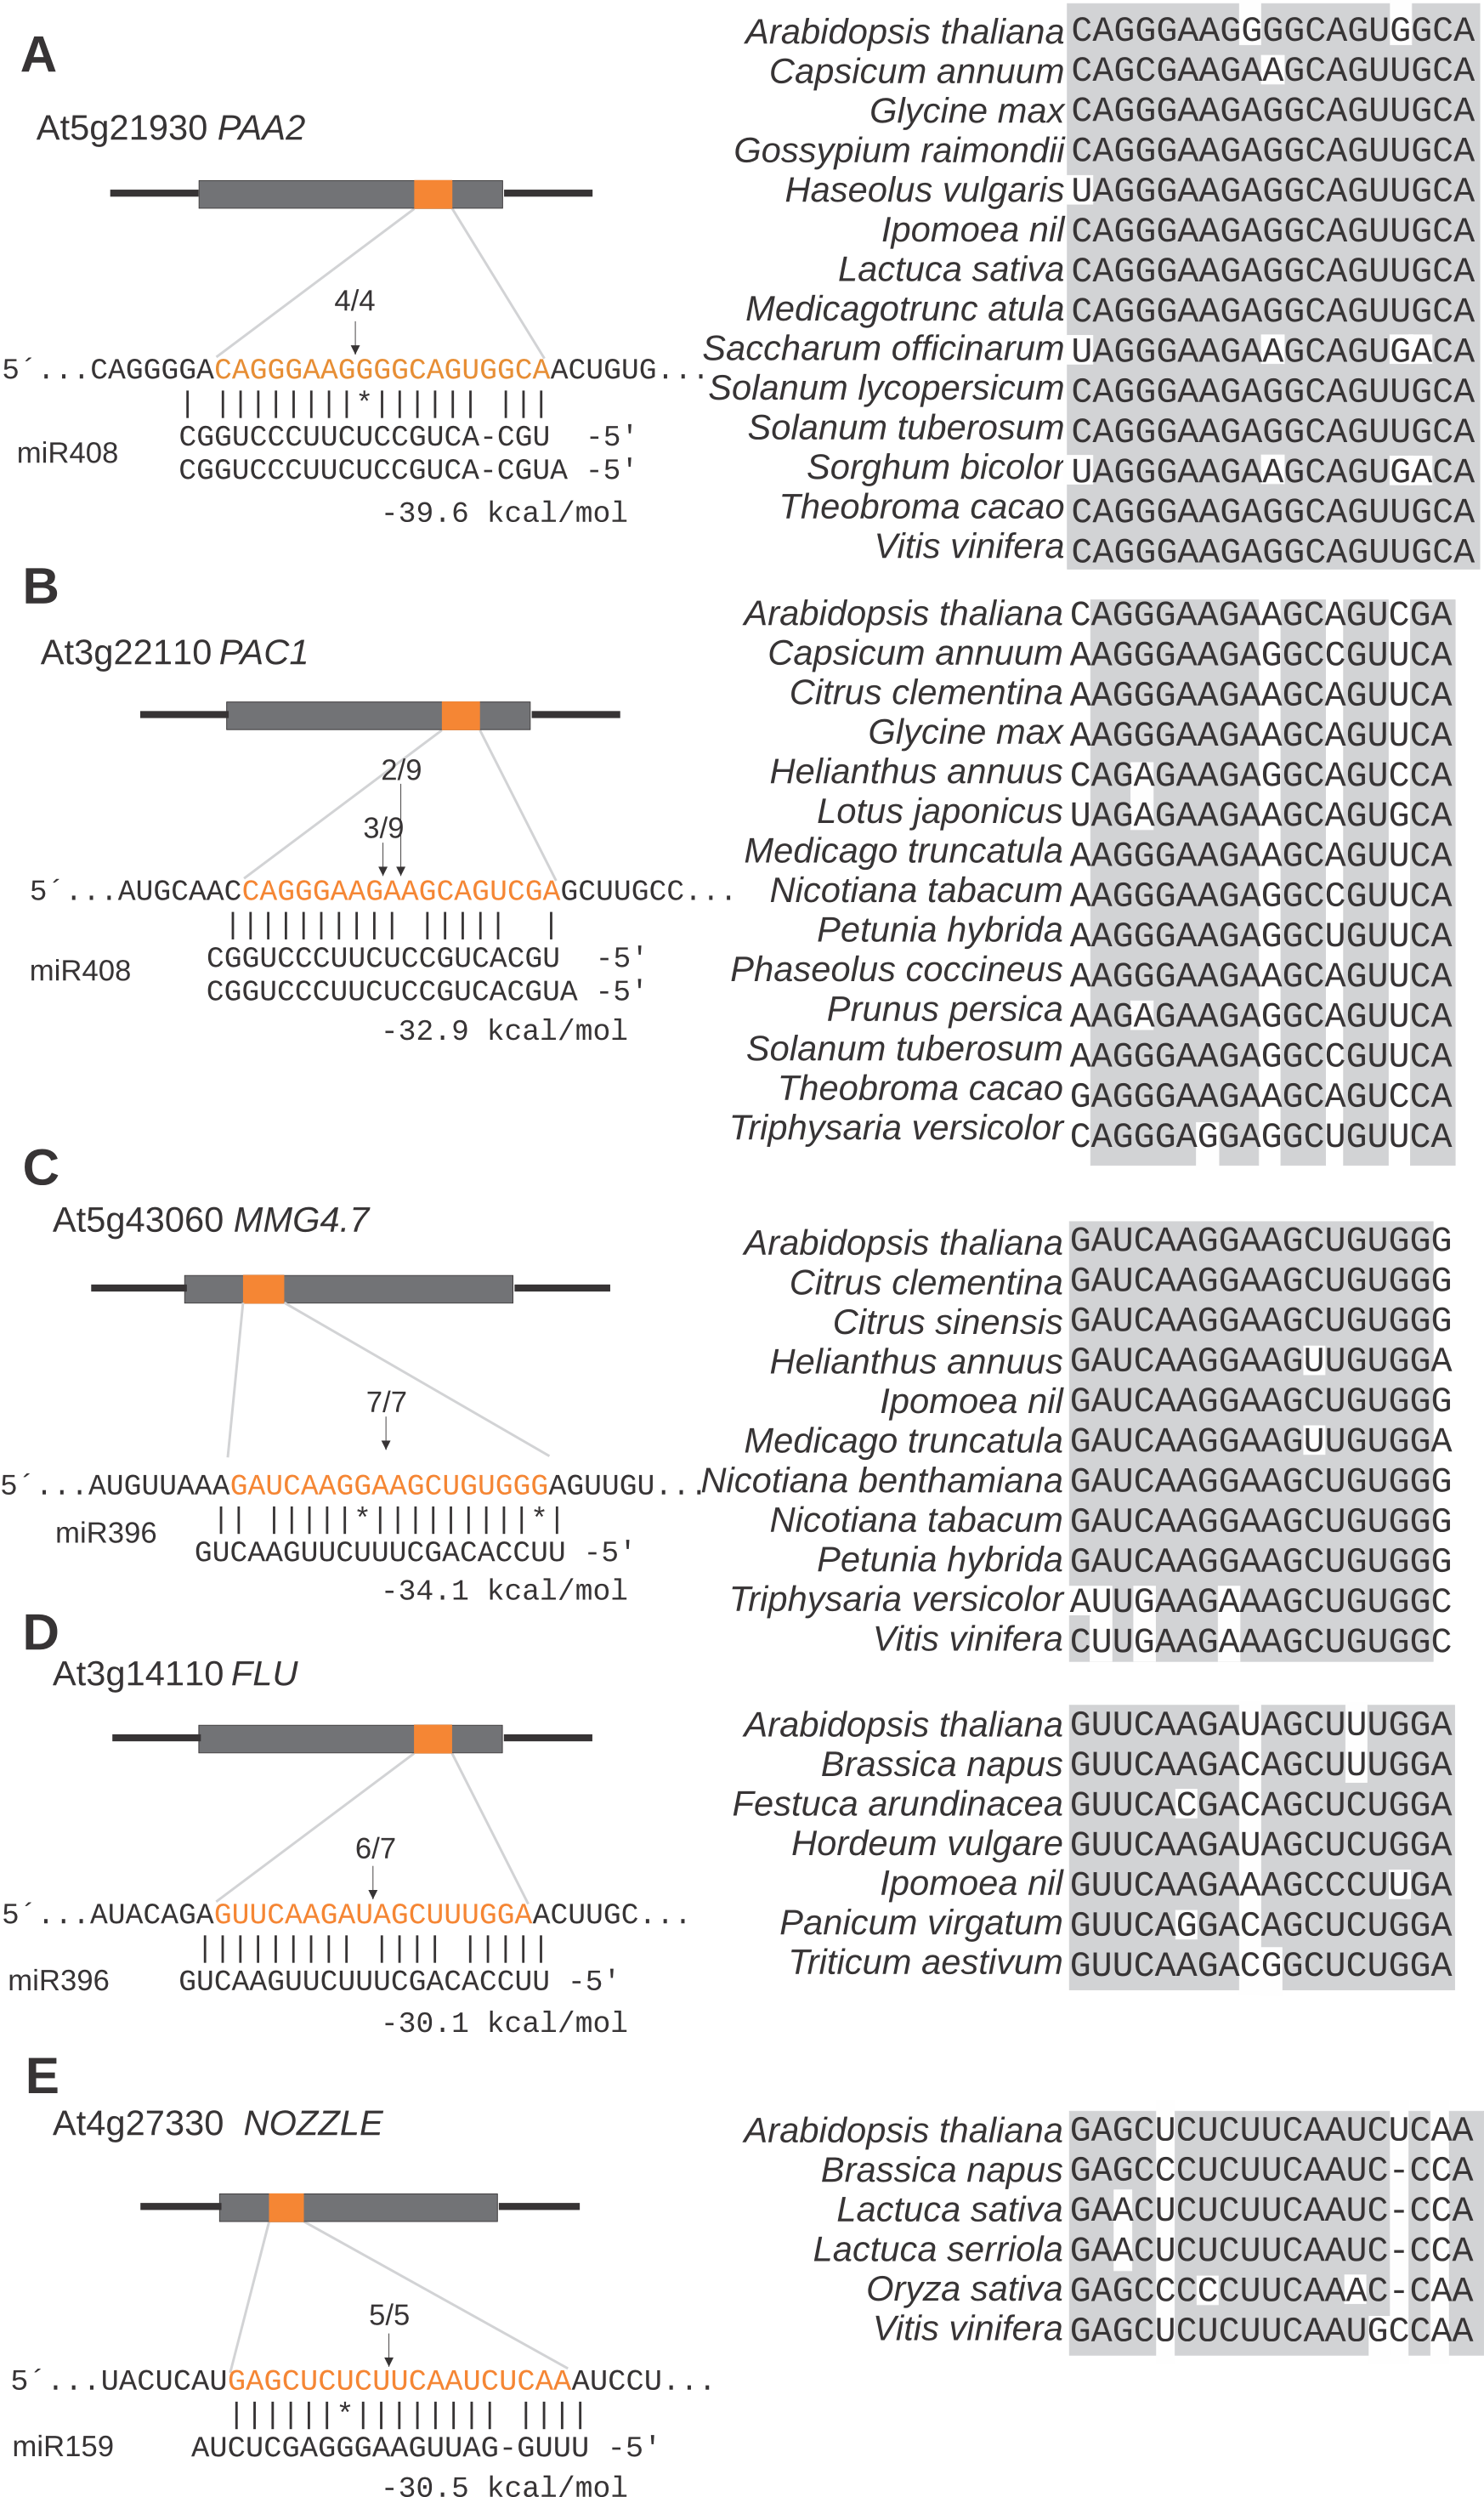
\includegraphics[width=0.7\textwidth]{NAR_fig4.png}
    \caption[Nuevos genes blanco validados en \textit{A. thaliana}.]{
    \textbf{Nuevos genes blanco validados en \textit{A. thaliana}.}
    El alineamiento entre el miARN y los nuevos genes blanco identificados se muestran en la izquierda.
    La conservación evolutiva de la secuencia del sitio reconocido por el miARN en las especies seleccionadas se muestra a la derecha. La figura muestra las interacciones del miR408 con PAA2
    \textbf{(A)}, miR408 con PAC1 \textbf{(B)}, miR396 con MMG4.7 \textbf{(C)}, miR396 con FLU \textbf{(D)}, miR159 con NOZZLE \textbf{(E)}.
    Las flechas marcan el sitio de corte determinado por 5’RACE-PCR y los números indican la frecuencia de clonadao de cada fragmento.}
    \label{fig:NAR_fig4}
\end{figure}


\subsection{Identificación de nuevos genes blanco permitiendo interacciones G-U.}

Los genes blanco identificados utilizando la estrategia descrita anteriormente, tienen varios "mismatches" y "bulges" con sus miARNs, lo que puede ayudar a explicar por que se perdieron en trabajos anteriores. 
También notamos que muchas de estas nuevas interacciones miARN-gen blanco contenían posiciones que variaban alternadamente entre G-C y G-U en distintas especies.
Como consideramos G-U como "mismatch" en nuestra búsqueda inicial, decidimos realizar nuevamente la búsqueda con los miARNs consenso de 18nt pero permitiendo ahora 4 "mismatches", donde al menos uno de ellos tiene que ser del tipo G-U.
Esta búsqueda permitiría interacciones miARN-gen blanco con sólo 14 bases apareadas perfectamente.

Para compensar el uso de estos parámetros relajados en términos de "mismatches", requerimos que el gen blanco aparezca en al menos 10 especies distintas para aumentar la especificidad (Figura \ref{fig:NAR_fig5} A).
Encontramos 125 potenciales genes blanco en \textit{A. thaliana} teniendo en cuenta este criterio (Figura \ref{fig:NAR_fig5} A) y 34 de ellos no aparecían en las búsquedas anteriores.
El gen blanco CSD2 regulado por el miR398, que no apareció anteriormente, fue detectado con estos parámetros. 

Luego examinamos el último grupo de potenciales genes regulados por miARNs que estaban realizando funciones auxiliares a los genes blanco ya descritos para cada miARN. 
Y encontramos que el miR167 que regula factores de respuesta a auxina (ARFs), también regulaba potencialmente a un gen denominado IAA-ALANINE RESISTANT 3 (IAR3) (Figura \ref{fig:NAR_fig5} B y C), que está involucrado en el control de niveles libre de auxina \citep{Davies1999,Rampey2004}.

IAR3 en Arabidopsis tiene 3 "mismatches" con respecto al miR167, pero en la posición 12 de la interacción miARN-gen blanco, hay una interacción G-U en varias especies (Figura \ref{fig:NAR_fig5} B y C).
La técnica de 5’ RACE PCR confirmó que el gen realmente era gen blanco del miR167 (Figura \ref{fig:NAR_fig5} C).

\begin{figure}[htbp!] 
    \centering    
    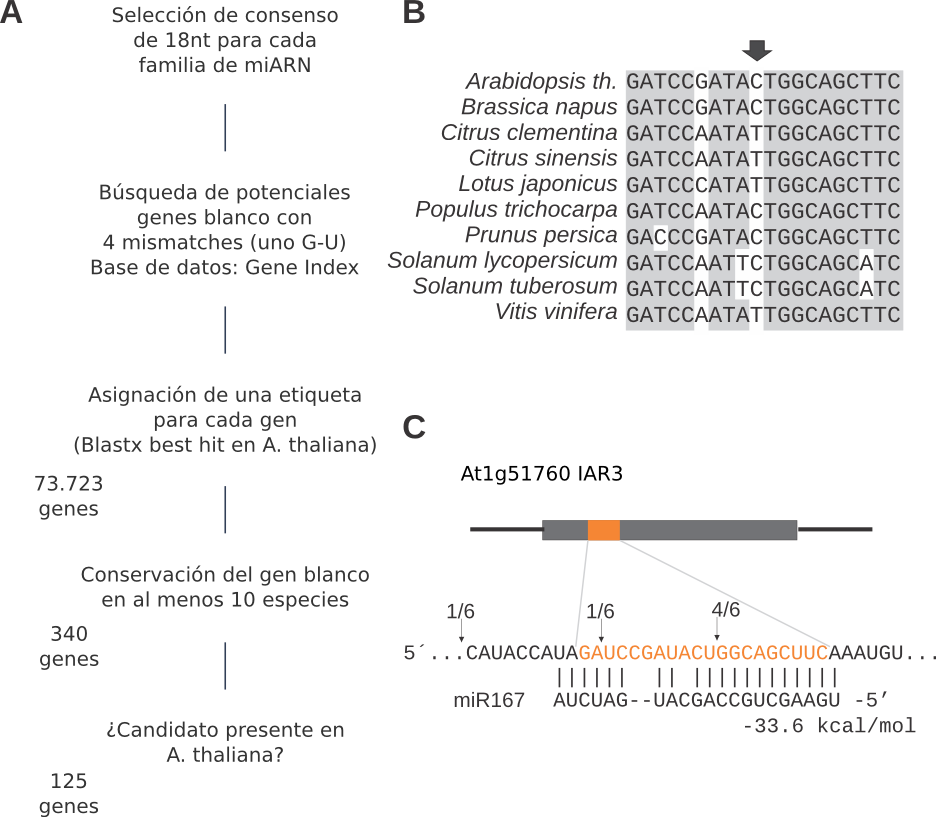
\includegraphics[width=0.8\textwidth]{NAR_fig5.png}
    \caption[Identificación de un nuevo gen blanco de miARN]{
    \textbf{Identificación de un nuevo gen blanco de miARN, relajando los parámetros de interacción pero incrementando el parámetro de conservación evolutiva.}
    \textbf{(A)} Esquema de la estrategia modificada para identificar genes blanco de miARNs.
    \textbf{(B)} Conservación del sitio blanco reconocido por el miARN en distintas especies.
    La flecha indica una variación de G-C o G-U con el miARN dependiendo de la especie.
    \textbf{(C)} Alineamiento en \textit{A. thaliana} del gen blanco IAR3 con el miR167. La flecha indica la posición del corte indicada por 5’RACE-PCR y el número indica la frecuencia de clonado de cada fragmento.}
    \label{fig:NAR_fig5}
\end{figure}


\subsection{Identificación de genes blanco específicos de \textit{Solanaceae}.}

Pensamos que la estrategia mostrada también se puede utilizar para encontrar genes blanco presentes específicamente en un grupo de especies relacionadas.
Por lo tanto intentamos demostrar esto, encontrando potenciales genes blanco específicos de la familia de \textit{Solanaceae}. 

Elegimos esta familia en particular, ya que 6 especies estaban bien representadas en la biblioteca utilizada.
La relación señal/ruido entre los genes blanco y las secuencias al azar era más de 2 cuando el filtro empírico o de conservación (en al menos 3 de las 6 especies \textit{Solanaceae} ) fueron aplicados (Figura \ref{fig:NAR_fig6} A).
Curiosamente, al aplicar ambos filtros dio como resultado una relación señal/ruido por encima de 6 (Figura \ref{fig:NAR_fig6} A), confirmando nuestros previos hallazgos de que ambos filtros mejoran la detección de genes blanco de miARNs.

Encontramos 132 potenciales genes blanco presentes en al menos 3 especies \textit{Solanaceae}. De este grupo, 41 genes no fueron detectados en otras especies (Figura 6B).
El gen blanco más común fue la metalotioneína MT2A, presente en las 6 \textit{Solanaceae}, como potencial gen blanco del miR398, mientras que MT2B, homólogo de este gen, fue detectado en 5 especies (Figura \ref{fig:NAR_fig6} B-D).

Luego, aprovechamos las plantas transgénicas de tabaco que contienen un transgén 35S.mir398 (A.F. Lodeyro, N. Carrillo y J.F. Palatnik resultados no publicados) y chequeamos la expresión de estos genes.
Encontramos que CSD2, un gen blanco conservado del miR398, disminuía su expresión > 10 veces en las plantas transgénicas 35S:miR398 comparadas con la planta salvaje (Figura \ref{fig:NAR_fig6} E).
Curiosamente, observamos que tanto MT2A como MT2B  disminuyeron sus niveles de transcripción > 5 veces en estas plantas (Figura \ref{fig:NAR_fig6} E).
Estos resultados concuerdan con la regulación de MT2A y MT2B por el miR398, aunque no necesariamente demuestra una interacción directa.
Además, estos resultados demuestran que los genes blanco presentes en un grupo específico de especies pueden ser encontrados utilizando esta estrategia.
Estos experimentos en tabaco los realizó la Dra. Anabella F. Lodeyro, que pertenece al grupo del Dr. Nestor Carillo del IBR.

\begin{figure}[htbp!] 
    \centering    
    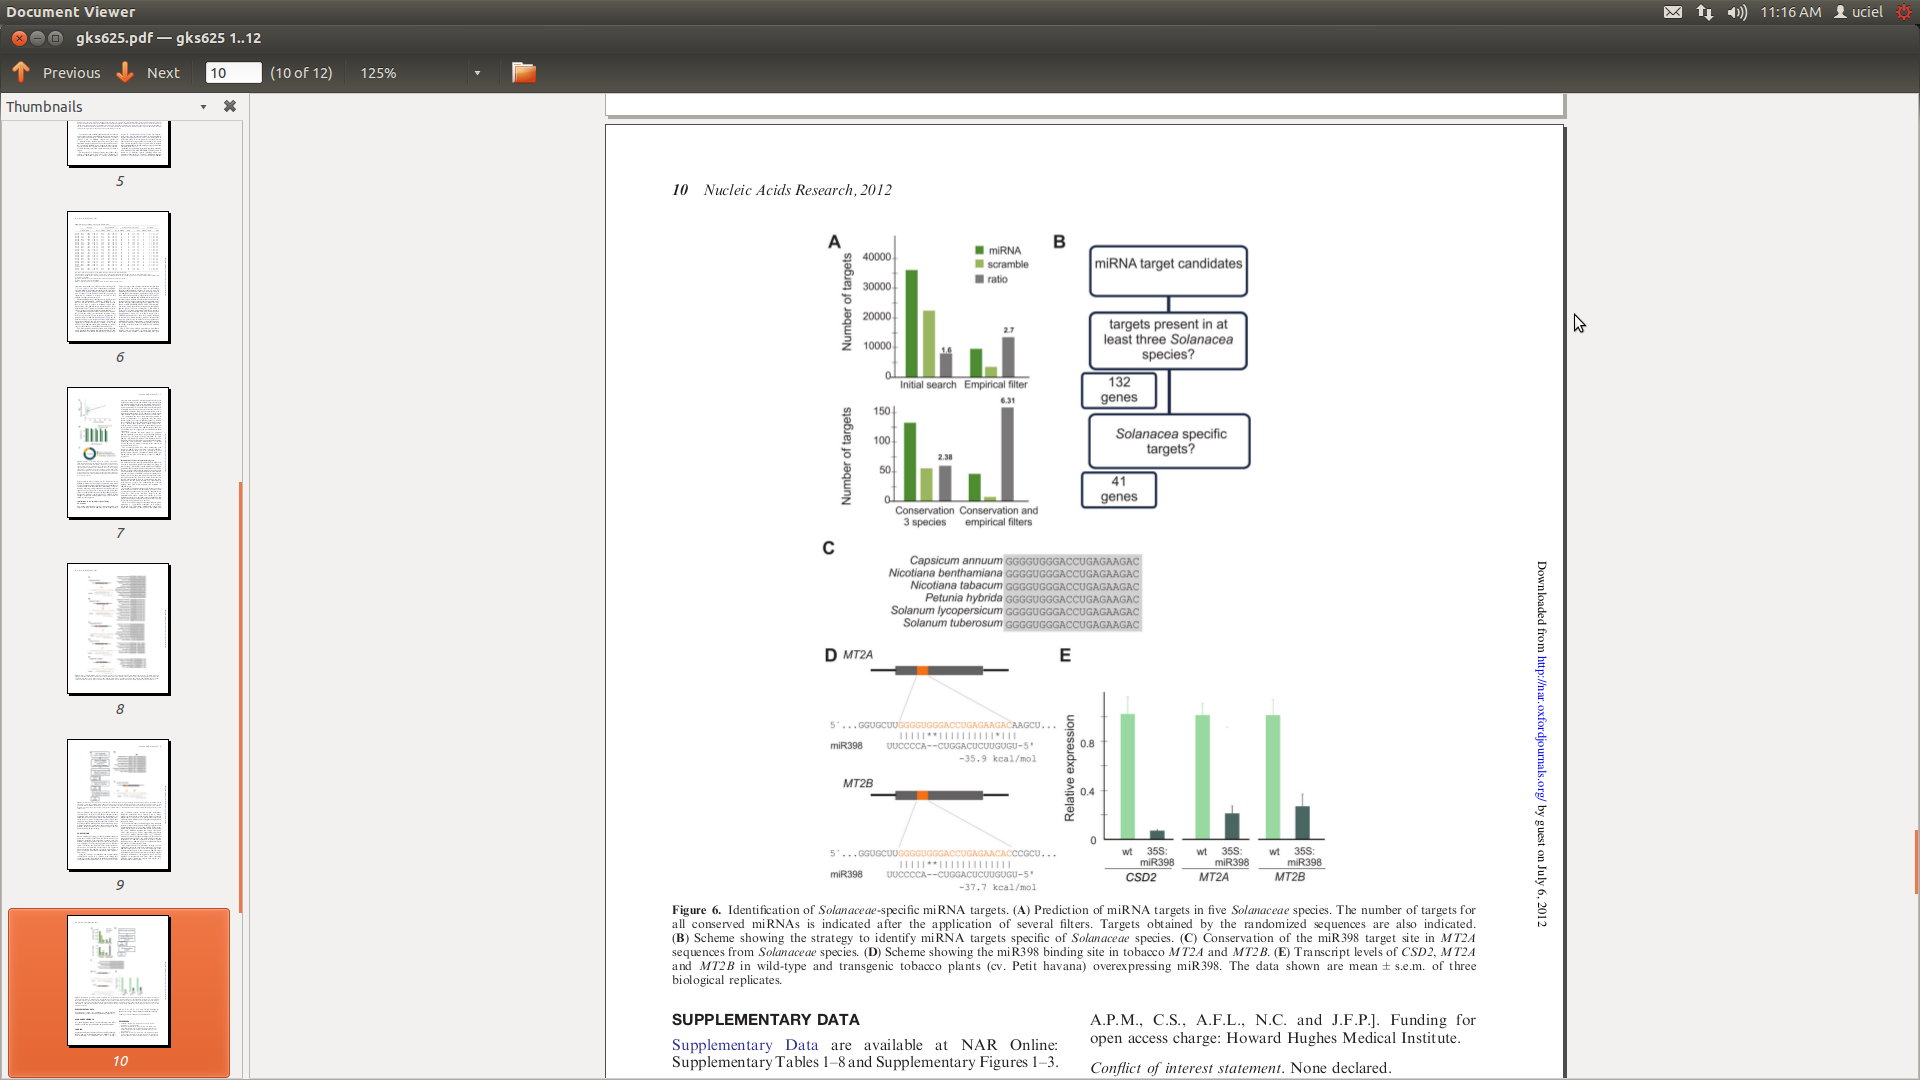
\includegraphics[width=0.7\textwidth]{NAR_fig6.png}
    \caption[Identificación de genes blanco de miARN, específicos de \textit{Solanaceae}]{
    \textbf{Identificación de genes blanco de miARN, específicos de \textit{Solanaceae}.}
    \textbf{(A)} Predicción de genes blanco de miARN en cinco especies de \textit{Solanaceae}.
    El número de genes blanco de todos los miARNs conservados juntos se muestra luego de aplicar distintos filtros.
    También se muestran los genes blanco obtenidos a partir de las secuencias al azar.
    \textbf{(B)} Esquema que muestra la estrategia para identificar genes blanco específicos de \textit{Solanaceae}.
    \textbf{(C)} Conservación del sitio reconocido por el mir398 con MT2A específico de \textit{Solanaceae}.
    \textbf{(D)} Esquema que muestra el sitio de unión entre el miR398 y MT2A y MT2B.
    \textbf{(E)} Niveles de transcriptos de CSD2, MT2A y MT2B en plantas salvajes y plantas transgénicas de tabaco (cv Petit havana) que sobreexpresan el miR398.  }
    \label{fig:NAR_fig6}
\end{figure}


\subsection{comTAR: una herramienta para la predicción de genes blanco regulados por miARNs en plantas.} 

A partir de la estrategia descrita en el capítulo anterior, que fue utilizada para encontrar y validar experimentalmente genes blanco regulados por miARNs en \textit{A. thaliana}, desarrollamos una herramienta web denominada comTAR\footnote{http://rnabiology.ibr-conicet.gov.ar/comtar} (Conserved plant miRNA target prediction tool) \citep{Chorostecki2014}.
La misma se puede utilizar para predecir potenciales genes blanco regulados por miARNs en plantas y está basada en la conservación evolutiva del par miARN-gen blanco con un número relajado de "mismatches".
ComTAR permite distintas opciones/parámetros de búsqueda que pueden ser modificados por el usuario:

\begin{itemize}
    \item Filtro de mismatch: Solamente un "mismatch" está permitido entre la posición 1 y la 11 de la secuencia del miARN consenso. (Sí/No).
    \item Corte por energía de hibridación: Se define que un gen blanco es predicho si la mínima energía de hibridación está por debajo del corte elegido.
    \item El número mínimo de especies donde una misma etiqueta está presente para un miARN particular.
\end{itemize}

Además con la herramienta comTAR se pueden realizar diferentes búsquedas, pudiendo elegir entre distintas opciones que más se ajustan a la necesidad del usuario.

\subsubsection{Realizar la búsqueda de potenciales genes blanco de miARN}
Esta es la búsqueda por defecto.
El usuario puede realizar la búsqueda de genes blanco de miARNs conservados.
En la primer pantalla se muestra los potenciales genes blanco para un miARN dado (Figura \ref{fig:comTAR_find_targets}), con una breve descripción del gen, la familia a la que pertenece y además en cuantas y cuáles especies está presente.
También, para cada especie detectada, se tiene acceso por pantalla al alineamiento del miARN-gen blanco, la energía de hibridación y los filtros empíricos de interacciones conocidas del par miARN-gen blanco (Figura \ref{fig:comTAR_fig2}).

\subsubsection{Realizar la búsqueda de familias de potenciales genes blanco de miARN}
Debido a que los miARNs en plantas en general regulan genes que codifican a proteínas de las misma familias, la herramienta tiene otra funcionalidad donde permite la búsqueda de genes agrupados por familias en vez de agruparlos por TAG.
De este modo genes en distintas especies con diferentes etiquetas, pero que pertenecen a la misma familia pueden ser detectados como familias de potenciales genes blanco de miARNs conservados.

\subsubsection{Realizar la búsqueda de un gen de interés para ver si es potencial gen blanco de algun miARN conservado}

El usuario puede introducir una etiqueta de locus en particular (tanto de Arabidopsis como el "gene ID" del Phytozome) y se identifica si este gen en particular puede ser un potencial gen blanco de algun miARN y además se muestra en cuantas especies se detecta.
En Arabidopsis se utiliza el LocusID como identificador, mientrás que en Phytozome este identificador varía según la especie y se puede ver la precedencia de cada especie en el sitio de Phytozome.

\subsubsection{Realizar la búsqueda de un miARN nuevo}
En esta parte del programa el usuario puede realizar la búsqueda de nuevos ARNs pequeños teniendo en cuenta que la secuencia introducida tiene que ser de 18nt de largo (posiciones 2-19).
Luego de la búsqueda, se da un link al usuario y después de unas horas, cuando haya sido procesado el cálculo, el usuario puede entrar a ese link y navegar los resultados por pantalla.

\begin{figure}[htbp!] 
    \centering    
    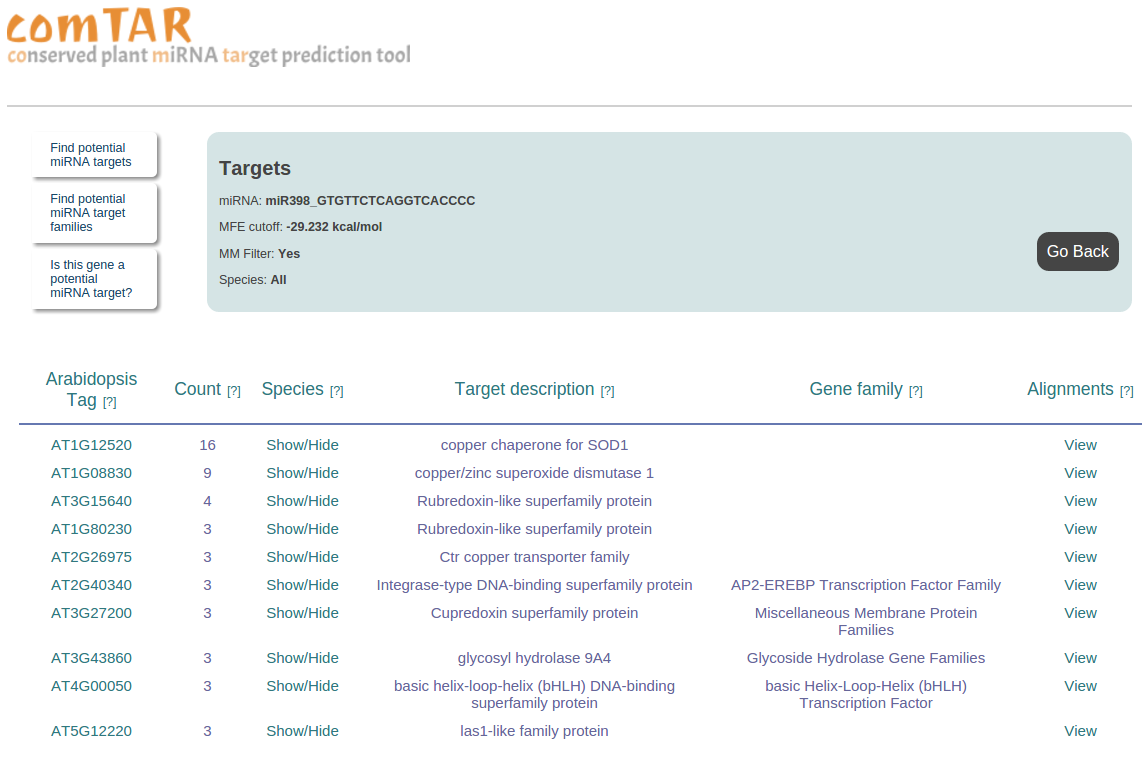
\includegraphics[width=1\textwidth]{comTAR_find_targets.png}
    \caption[Resultados del comTAR para el miR398]{
    \textbf{Resultados de la búsqueda de comTAR, con parámetros por defecto para el miR398}}
    \label{fig:comTAR_find_targets}
\end{figure}

\begin{figure}[htbp!] 
    \centering    
    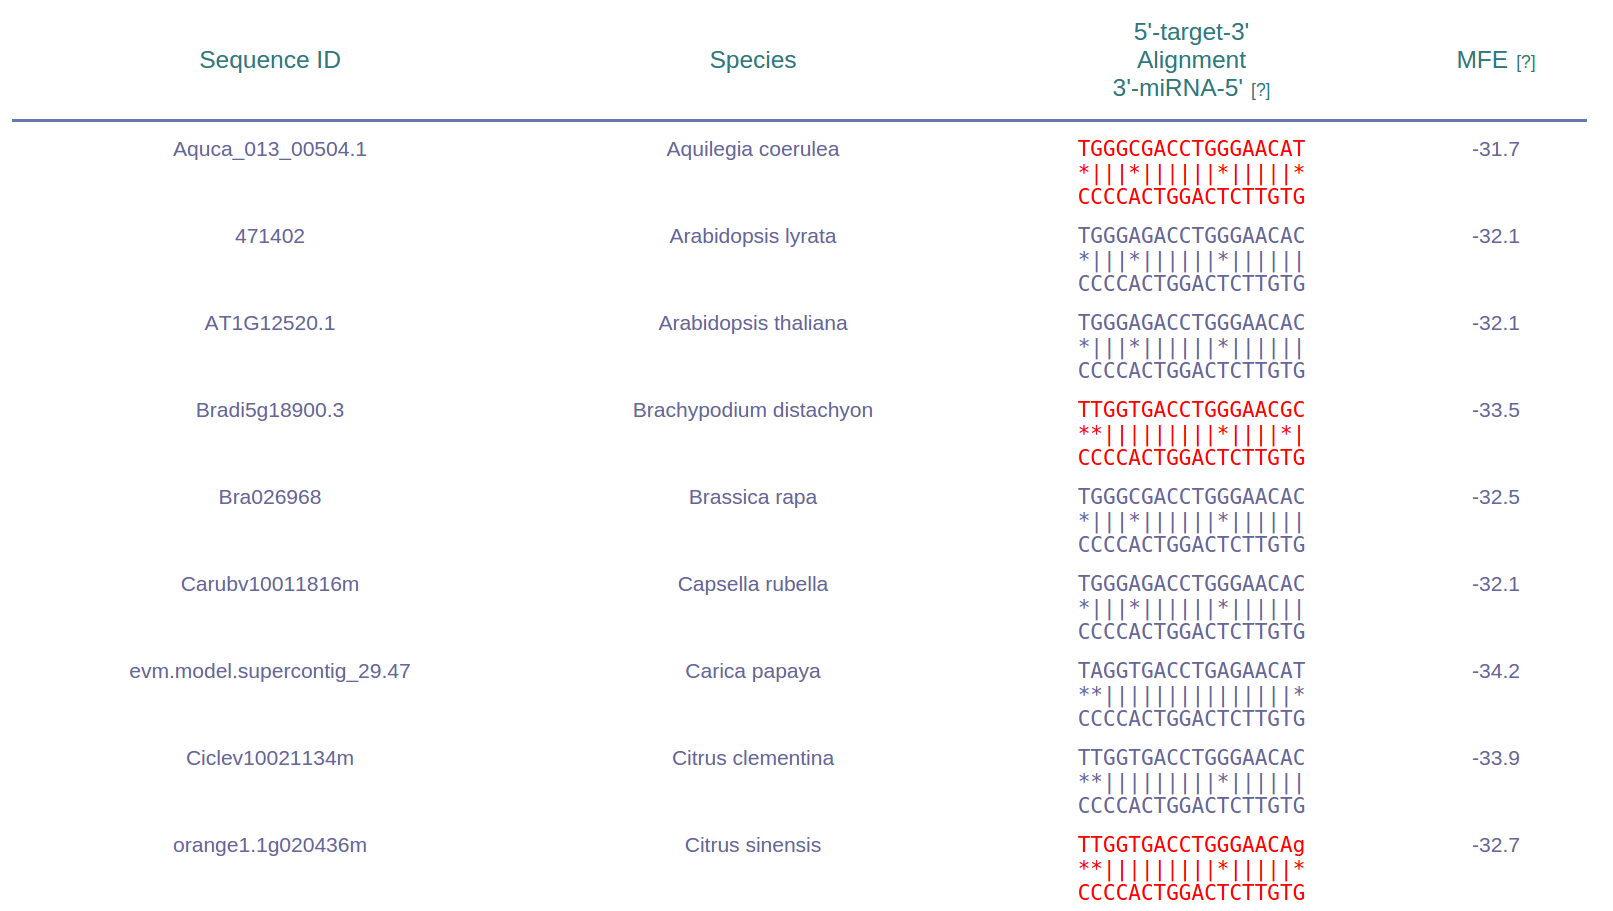
\includegraphics[width=1\textwidth]{comTAR_fig2.png}
    \caption[Captura de pantalla de comTAR]{
    \textbf{Captura de pantalla de comTAR}
    Parte de la salida de comTAR mostrando el par miR398/SOD1 (At1g12520) en diferentes especies}
    \label{fig:comTAR_fig2}
\end{figure}


\section{Conclusiones}

En este primer capítulo diseñamos una estrategia para identificar genes blanco regulados por miARNs en plantas, basado en la conservación evolutiva del par miARN-gen blanco.
El enfoque requiere que la interacción miARN-gen blanco, pueda ocurrir en el contexto de un conjunto mínimo de parámetros que interactúan en diferentes especies pero la secuencia del gen blanco en sí, no necesariamente tiene que estar conservada.
Además, nuestro enfoque permite ajustar el número de especies requeridas como un filtro para realizar la búsqueda con diferentes sensibilidades y relaciones señal/ruido.

Utilizando esta estrategia identificamos y validamos experimentalmente nuevos genes blanco en \textit{A. thaliana}, a pesar de que este sistema ya había sido estudiado en detalles en distintos enfoques genómicos a gran escala (\citep{Allen2005207,JonesRhoades2004787,Addo-quaye2009a,German2008,Rajagopalan2006,Schwab2005517}).
Validamos nuevos genes blanco con funciones relacionadas con genes blanco ya conocidos.
El miR159 regula factores de transcripción de la familia MYB y NOZZLE (validado por nosotros en \citep{Chorostecki05072012})  que están involucrados en el desarrollo del estambre y polen\citep{Millar2005,Biology1999,Yang1999,pmid17916625}.
El miR408 regula el transportador de cobre PAA2 (validado por nosotros en \citep{Chorostecki05072012}), como también proteínas de unión a cobre \citep{JonesRhoades2004787,German2008,Schwab2005517,pmid15258262}
El miR167 regula a la familia ARFs \citep{Rhoades2002513,pmid17021043} y a IAR3 (validado por nosotros en \citep{Chorostecki05072012}), y ambos participan en el control de niveles y actividad de auxinas \citep{Davies1999,pmid15491917}.

Además, tres de los nuevos genes blanco validados tienen "bulges" y los parámetros empíricos usualmente le otorgan una gran penalidad a ellos, que puede llegar a ser el doble que un mismatch regular \citep{JonesRhoades2004787}, 
Sin embargo es probable que genes blancos con "bulges" asimétricos sean más frecuente de lo que se pensaba previamente en plantas.
Es por esto que el enfoque ofrece una estrategia alternativa a otras predicciones que se basan en parámetros empíricos del par miARN-gen blanco \citep{Allen2005207,JonesRhoades2004787,citeulike:8816489,Fahlgren_chapter}.
Una ventaja de la estrategia presentada es que la interacciones miARN-gen blanco conservadas probablemente participen en procesos biológicos relevantes.
Además, esta estrategia puede ser fácilmente modificada para incorporar datos de otras bibliotecas, y/o para realizar la búsqueda de genes blanco presentes en un grupo específico de especies de plantas como se demostró para \textit{Solanacea}.

Por último desarrollamos una herramienta web denominada comTAR\footnote{http://rnabiology.ibr-conicet.gov.ar/comtar} para predecir potenciales genes blanco regulados por miARNs en plantas.
Esta herramienta, es flexible y se puede utilizar también potenciales genes blanco para nuevo ARN pequeños o para buscar familias de potenciales genes blanco de miARNs en plantas. 

Esta parte del trabajo de Tesis fue publicado en la revista Nucleic Acid Research \citep{Chorostecki05072012} y en la revista Bioinformatics \citep{Chorostecki2014}.
La validación experimental de los genes blanco regulados por miARNs detectados con la estrategia, fueron realizadas por colegas del laboratorio.
En particular, la validación de los genes blanco de \textit{A. thaliana} por 5' RACE PCR modificada, las realizó Valeria Crosa.
Y los experimentos en tabaco los realizó la Dra. Anabella Lodeyro.
